% Revision information
% $Author$
% $Date$
% $Revision$
%---------------------------------

\documentclass[a4paper,10pt]{scrartcl}
\usepackage{graphicx}
\usepackage{fancyhdr}
\pagestyle{fancy}
\chead{\textsc{Confidential}}
\rhead{}
\lhead{}
\usepackage{lastpage}
\cfoot{\thepage\ of \pageref{LastPage}}

%opening
\title{Tomography of dynamic processes using hierarchical acquisition protocols}
\author{A. Kaestner and Who. Else}

\begin{document}

\maketitle

\begin{abstract}
For dynamic processes the local composition of the sample varies with time. When the time constant of the observed system is close to the time required to complete tomographic scan so called motion artifacts will appear. These artifacts appear as indistinct structures in the reconstructed image. We propose a method to reduce the impact of these artifacts by altering the acquisition protocol from a traditional angular incremental rotation to a hierarchical decomposition of the scan arc.
Numerical validation experiments and reconstructions of sand columns illustrate the advantage of the proposed protocol. An additional feature of the proposed protocol is that time series of the process can be reconstructed from a single scan.
\end{abstract}

\section{Introduction}
The scan times for neutron tomography are often very long compared to for example medical X-ray CT devices. This makes the tomography of dynamic processes difficult. A further difference to the medical application the temporal changes are at the best monotone instead periodic. This makes acquisition protocols based on incremental gantry angles less applicable\cite{li2006}.

Here a different acquisition protocol is proposed. It is based on the scale based binary decomposition of the scan trajectory.
The initial idea behind non-incremental acquisition protocols was to guarantee that the data always is complete and that the scan can be terminated at any time (reference needed). This protocol still aimed at reconstruction of a single tomogram.
A further feature of the proposed scan strategy is that a 4D image can be reconstructed. This can be achieved since at any time during the scan a set of N projections representing the complete information for a reconstruction can be extracted.

\section{Method}
\subsection{Introduction}
The basic idea is to decompose the scan into a pattern that forms binary tree. Two basic requirements on the tree are:
\begin{itemize}
 \item Each branch of the tree shall contain sufficient information to reconstruct an image.
 \item Each branch shall represent a given time interval of the scan and two branches on the same level are not allowed to overlap in time.
\end{itemize}
This implies that the sample must rotate back and forth during the scan. A consequence of these conditions on the scan tree is that the measurement can capture temporal information. The number of time steps depends on the level of the root nodes, figure \ref{fig_binarytree}.
\begin{figure}
 \centering
 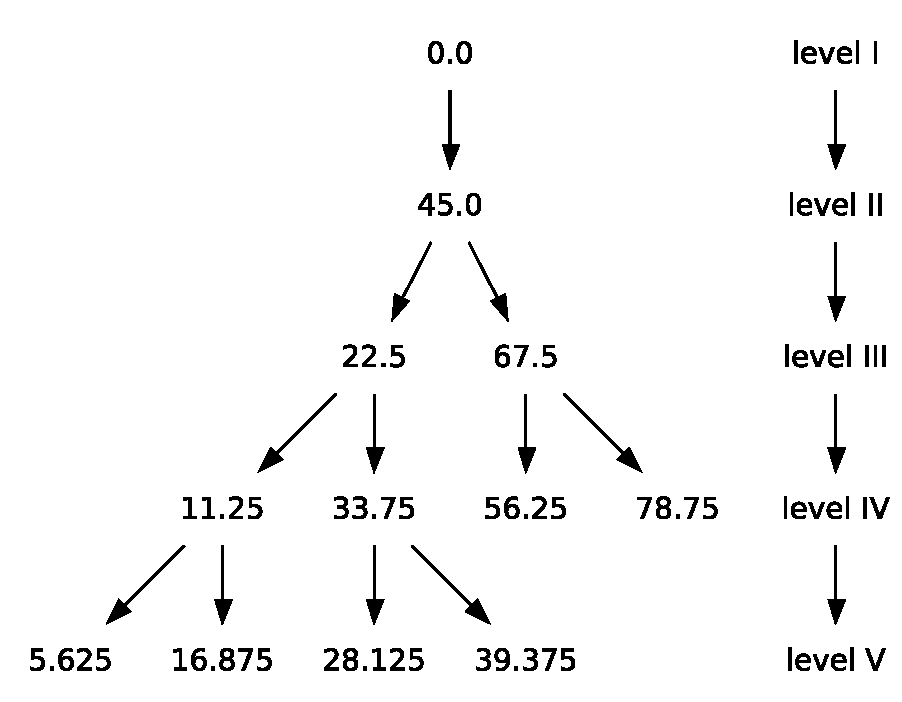
\includegraphics[width=0.5\textwidth]{figures/tree}
 \caption{A first tree, does not satisfy the completeness condition.}\label{fig_binarytree}
\end{figure}

\subsection{Building the scan tree}\label{sec_ScanTree}
This is the core of the method. The tree must be well-balanced both in terms of coverage and of the scan arc and in time. A known scan strategy that achieves a reasonable tree balance is based in on the Greek golden ratio\cite{goldenratio}.  

\subsection{Down sampling}
The quality of the reconstructed image depends on the number of projections used and the size of the projections. This relation is determined by the sampling theorem \cite{kak88}. A suggestion would be to down-sample the projections to match the reconstruction of M time steps. The sampling theorem here implies a uncertainty relation between temporal and spatial resolution.

\subsection{Reconstruction}
The reconstruction of the projection data will be done with an in-house developed software. The reconstructor uses the filtered back-projection algorithm for parallel-beam geometry.

\section{Numerical validation}
The first validation of the method will be done using numerical projection data. The idea is to simulate the dynamic water movement in a three-dimensional structure. A complete test data set will contain a time series of three-dimensional image. These images will be feed to a forward projector that generates the projection data that will be used in the experiment.
\subsection{Models}

\subsection{Results}
\section{Experiments}
There is a possible pit-fall for experiments. The micro-vibrations induced by the turn-table may disturb the state of the sample. This still has to be investigated.
\subsection{Experimental setup}
It is not intended to modify the mechanical and electrical setup of the tomography platform installed on the beam-line. The only modifications are aimed at the control system. The control system must implement either the possibility to read turn-table positions from a file or to implement a module that computes the positions according to the method describe in section \ref{sec_ScanTree}.

\subsection{Samples}
\subsection{Results}
\section{Conclusions}

\bibliographystyle{plain}
\bibliography{../../../references}
\end{document}
